\section{Experiments}
\label{sec:experiments}

\paragraph{Locked evaluation protocol.}
Evaluation follows the \href{https://github.com/reeldemo/denoise-opt-meta/blob/master/paper/Unsupervised_Wavetable_Seam_Artifact_Repair_via_Hybrid_GA-PPO_Meta-Search_v10/EVAL_PROTOCOL.md}{v10.1 evaluation protocol}.
Primary metric: $R_{\mathrm{blend}}$ ($\alpha{=}0.7$).
Search objective: $J$ as in~\eqref{eq:outer-obj} ($\lambda{=}0.02$).
Champ gate: strictly beat frozen Noise2Noise corrupt$\to$corrupt holdout $R_{\mathrm{blend}}$.
Secondary: SNR, SDR, wrap-jump, seam-local edge RMSE; debug keys include pure $R_{\mathrm{seam}}$ and whole-curve $R$.
Holdout seed \texttt{20260719}. Search seed \texttt{1902771841}. N2N train seed \texttt{424242}.
We report the hybrid\_lstm freeze plus holdout / multi-family / Factory+FX / AKWF / transfer benches.
PESQ/STOI stay out of scope on non-speech cycles. LibriSpeech and MUSDB are not used.
Venue: DSP / synthesis artifact repair (DAFx / AES / arXiv cs.SD).

\subsection{Dataset}
\label{sec:dataset}

\paragraph{Creation.}
The paper-facing evaluation corpus is a frozen draw from the same synthetic generator used by the CUDA search runner (\texttt{make\_batch}).
Each cycle has length $L{=}256$.
A two-harmonic sine is drawn with frequency $\sim\mathcal{U}(1,4)$ and phase $\sim\mathcal{U}(0,2\pi)$.
An open-wrap seam cliff of amplitude $\pm\mathcal{U}(0.08,0.43)$ is applied over $\texttt{SEAM\_W}{=}8$ samples at both ends.
Seam-boosted Gaussian noise (scale $0.02$ at the ends, $0.15\times$ in the mid-cycle) is added to form the engine input.
The ideal withholds the cliff and is used only as the scoring target $r^{\star}$ (never as a method output).
No-bake leaves the cracked engine unchanged and scores that unrepaired $x$ against the same $r^{\star}$.
Prolonged residual $R$ tiles each cycle $N{=}16$ times before the RMS ratio.
The holdout seed is \texttt{20260719} (distinct from the hybrid search seed \texttt{1902771841}).
The search campaign draws fresh i.i.d.\ batches from this generator and does not train on the frozen holdout tensors.
There is no supervised clean/noisy training split of studio audio.

\paragraph{Multi-family diversity ($\ge 20$ waveforms).}
Beyond the single sine{+}cliff holdout, Phase~3a scores methods on \textbf{20} generative draws: ten family variants (\texttt{sine\_cliff}, \texttt{harmonic\_fft}, \texttt{am\_fm}, \texttt{nonlinear}, \texttt{combo}, \texttt{triple\_mix}, \texttt{extreme\_overlay}, \texttt{open\_wrap\_bias}, \texttt{soft\_noise}, \texttt{wide\_seam}) $\times$ two seeds (\texttt{20260719} and \texttt{20260720}), batch 64 each ($128$ cycles per family; $1{,}280$ total).
These Python generative variants stress harmonic / AM--FM / nonlinear / overlay / open-wrap behavior of \texttt{make\_batch} and remain the primary SOTA matrix.
Separately, \texttt{export\_sound\_bench\_tiles} exports \textbf{20} Rust \texttt{sound\_bench} engine/ideal pairs (10 families $\times$ 2 seeds, $L{=}256$, byte-aligned with \texttt{generate\_sound} / \texttt{generate\_sound\_ideal}) scored under the same residual geometry as a secondary transfer block (Table~\ref{tab:rust-bench}).
Every method sees the same tensors per waveform.
\textbf{Primary classical comparison} is absolute prolonged $R$ against the non-AI board (no-bake, DualCosine, \texttt{seam\_fir3}, poly, fades, VA residuals; Section~\ref{sec:classical-board}).
The search objective is maximize $R$ toward the ideal sibling (best $R{=}1$).
DualCosine is one classical comparator and a PPO centering constant.
It is not the reward target.

\paragraph{Dataset statistics.}
Table~\ref{tab:dataset-stats} and Figures~\ref{fig:dataset-size}--\ref{fig:dataset-transfer-sizes} inventory every evaluation board used in this paper.
The primary procedural holdout is a frozen $4{,}096$-cycle metrics draw ($L{=}256$, $N{=}16$ tiles, seed \texttt{20260719}) plus a matched score batch of $64$ cycles (five consecutive seeds for classical mean$\pm$std).
Multi-family SOTA scores $20$ waveforms ($10$ families $\times$ $2$ seeds, batch $64$; $1{,}280$ cycles).
Wavetable-native boards use ReelSynth Factory+FX exports ($n{=}1{,}280$: $640$ dry + $640$ FX) and AKWF CC0 cycles ($n{=}1{,}280$) so Plot~4 corpus bars are comparable to multi-family ($1{,}280$).
Sci/eng transfer tiles $1{,}536$ periods across CWRU, MFPT ($n{=}256$), MIT-BIH, PTB-XL subset, and synthetic CNC/PMU.
Search never trains on the frozen holdout; N2N/seq baselines use disjoint train seeds \texttt{424242}/\texttt{424243}.
Artifacts: \href{https://github.com/reeldemo/denoise-opt-meta/tree/master/paper/Unsupervised_Wavetable_Seam_Artifact_Repair_via_Hybrid_GA-PPO_Meta-Search_v10/figures}{v10 dataset artifacts}.

\begin{table}[t]
  \centering
  \caption{Dataset statistics (evaluation boards).
    $L{=}256$ unless noted. Hours are raw source duration on disk where measurable, not tiled period count.
    Plot~4 compares ${\approx}1{,}280$-height boards only (multi-family / Factory+FX / AKWF / transfer).}
  \label{tab:dataset-stats}
  \setlength{\tabcolsep}{3pt}
  \begin{tabular}{@{}llp{0.42\columnwidth}@{}}
    \toprule
    Board & Size & Notes \\
    \midrule
    Holdout metrics & $4{,}096$ cycles & seed \texttt{20260719}; $N{=}16$ tiles \\
    Score batch & $64$ cycles & classical / favorite tables \\
    Multi-family SOTA & $1{,}280$ cycles & $10$ families $\times$ $2$ seeds $\times$ $64$ \\
    Factory+FX export & $1{,}280$ periods & $640$ dry + $640$ FX mid-tile extracts \\
    AKWF OA & $1{,}280$ periods & CC0 single-cycle WAVs \\
    Meta hybrid\_lstm & $1{,}200$ iters & $R_{\mathrm{blend}}{+}J$; seed \texttt{1902771841} \\
    CWRU & $256$ periods & $4$ MAT files; DE @12\,kHz \\
    MFPT & $256$ periods & shaft-rate windows \\
    MIT-BIH & $256$ periods & $10$ records @360\,Hz \\
    PTB-XL subset & $256$ periods & $94$ \texttt{*\_hr} @500\,Hz \\
    synth CNC / PMU & $256{+}256$ & procedural pilots \\
    \bottomrule
  \end{tabular}
\end{table}

\begin{figure}[t]
  \centering
  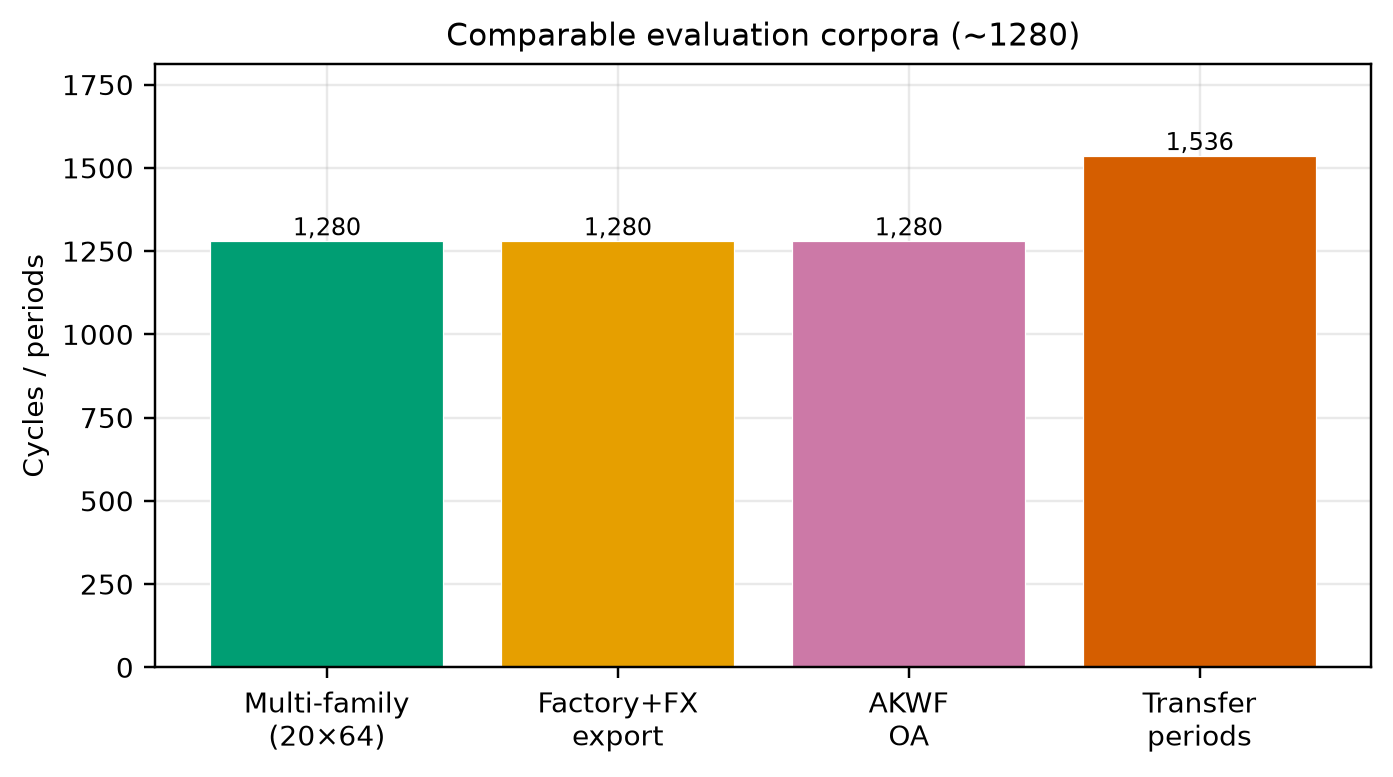
\includegraphics[width=\columnwidth]{figures/fig_dataset_size_overview.png}
  \caption{Corpus sizes across evaluation boards (cycles or periods).
    Holdout metrics draw, matched score batch, multi-family SOTA, factory/AKWF wavetable-native sets, and summed transfer periods.}
  \label{fig:dataset-size}
\end{figure}

\begin{figure}[t]
  \centering
  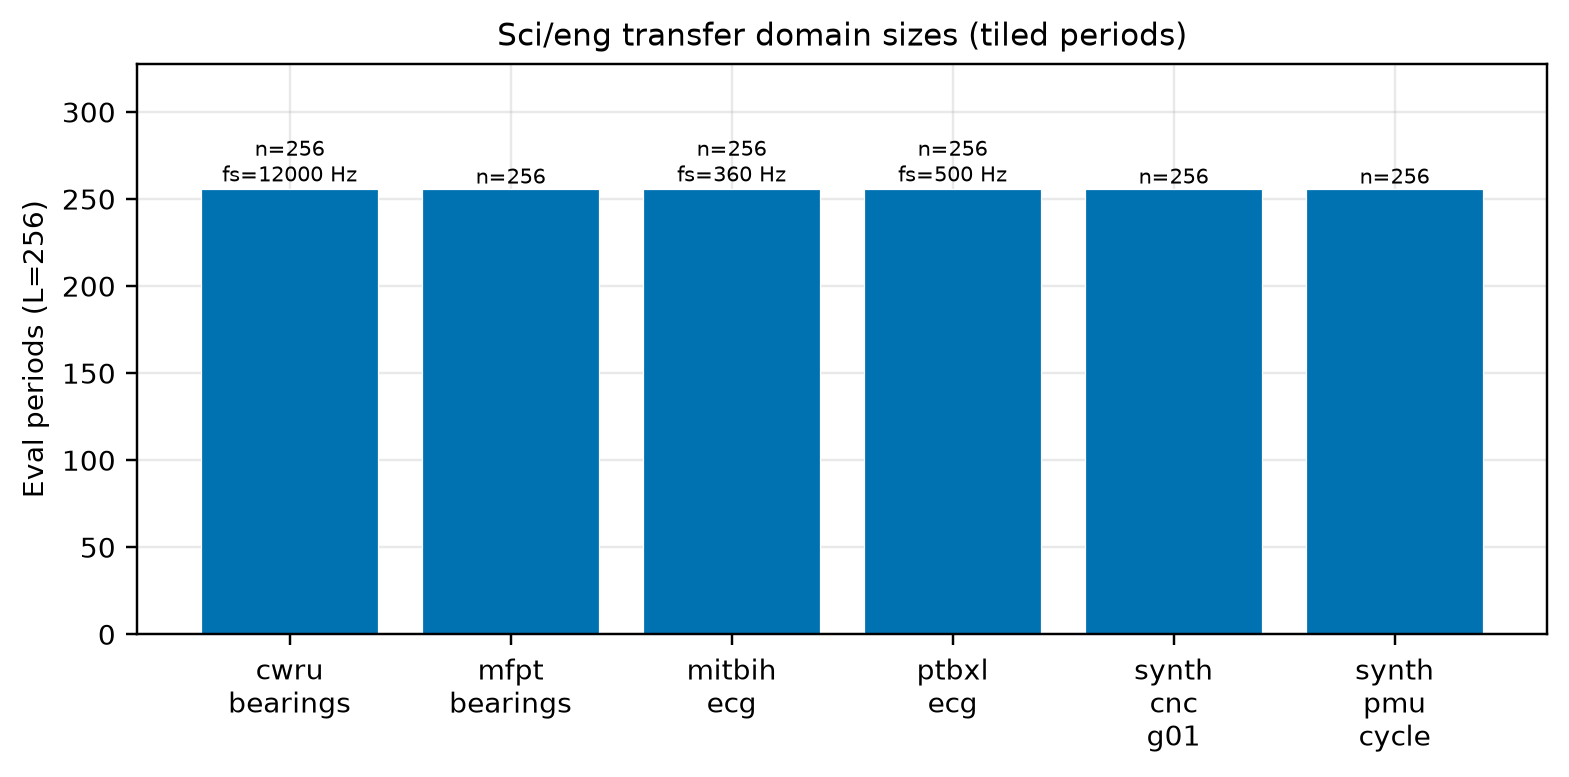
\includegraphics[width=\columnwidth]{figures/fig_dataset_transfer_sizes.png}
  \caption{Sci/eng transfer domain sizes: tiled eval periods at $L{=}256$ (with source $f_s$ where applicable).}
  \label{fig:dataset-transfer-sizes}
\end{figure}

\paragraph{Dataset metrics.}
A metrics draw of $4{,}096$ cycles under the holdout seed yields mean ideal RMS $0.721\pm0.016$, mean engine residual RMS $0.021\pm0.013$, and mean absolute wrap jump $|x_0-x_{L-1}|$ of $0.913\pm0.634$.
No-bake (passthrough) on that draw scores mean $R\approx0.971$.
Method tables use a matched score batch of $64$ cycles from the same seed (the \href{https://github.com/reeldemo/reelsynth/tree/main/brand/artifacts/canonical_eval_dataset}{canonical evaluation tensors}), five consecutive seeds for mean$\pm$std on the classical table, and the 20-waveform matrix for SOTA secondary metrics.
Figure~\ref{fig:dataset-distributions} summarizes the $4{,}096$-cycle metrics draw: ideal RMS clusters near $0.72$, wrap jumps span nearly three orders of magnitude (median $\approx 0.83$), and no-bake $R$ is high on easy tiles but falls below $0.91$ on the hardest decile of wrap jumps.
Figure~\ref{fig:intro-sine} is the documented sine-wrap edge case: a high-$|wrap|$ holdout tile where cliff modulation is visible, scored with DualCosine and the top neural favorite under the same residual $R$ (tile $R\approx0.9917$, favorite batch mean $R\approx0.991$).

\begin{figure}[t]
  \centering
  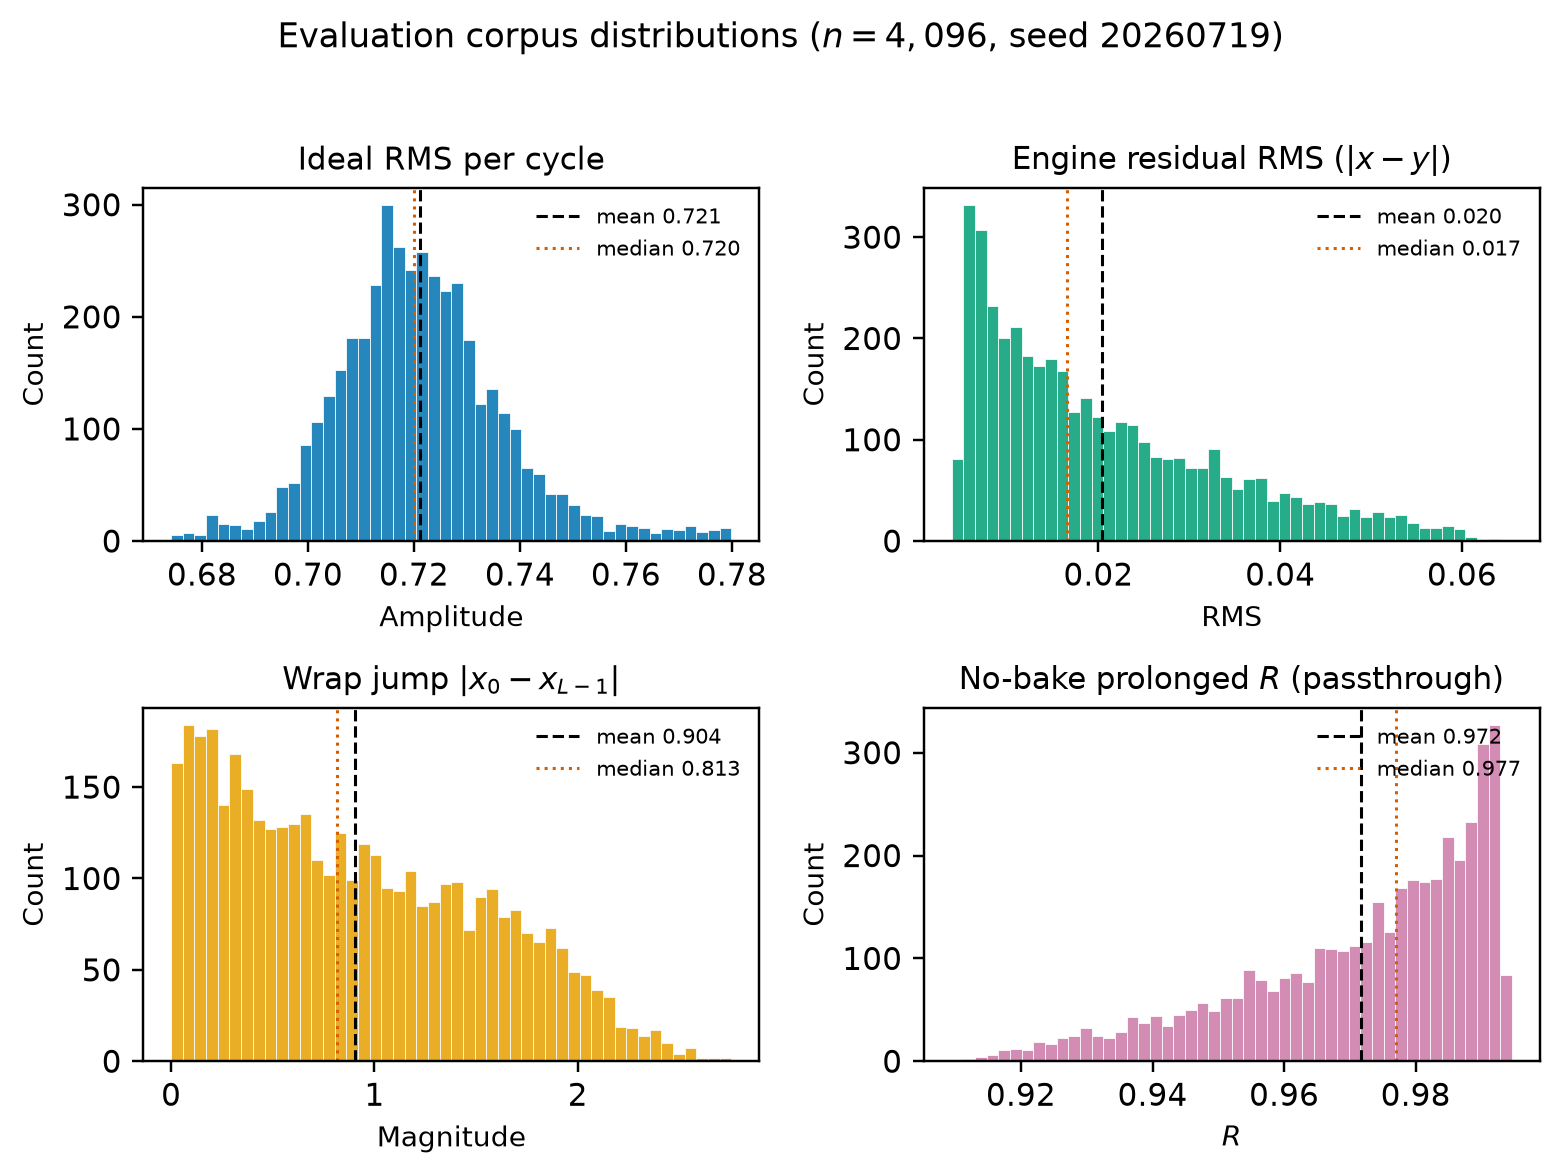
\includegraphics[width=\columnwidth]{figures/fig_dataset_distributions.png}
  \caption{Holdout distribution statistics (seed \texttt{20260719}, $n{=}4{,}096$ cycles).
    Distinguish: ideal sibling $r^{\star}$ (cliff withheld); no-bake $=$ unrepaired cracked engine (not $r^{\star}$); DualCosine $=$ one classical bake.
    Top left: ideal RMS per cycle.
    Top right: engine residual RMS before any bake.
    Bottom left: wrap jump magnitude $|x_0-x_{L-1}|$ (cliff hardness proxy).
    Bottom right: no-bake prolonged $R$ (passthrough, $x\mapsto x$).
    Dashed and dotted vertical lines mark mean and median.
    Hard-cliff reporting (Section~\ref{sec:results}) uses the top 10\% wrap-jump stratum where no-bake $R$ drops.}
  \label{fig:dataset-distributions}
\end{figure}

\paragraph{Hybrid search campaign (5,000-iteration freeze).}
A CUDA search tagged \texttt{PPO+GA+PBT+NAS+depth+MoE} runs with a large declared iteration budget (order $10^{5}$).
At the reported freeze (run \texttt{gpu-rl-arch-20260719T083019Z}, $\approx 6{,}922$ clean iters / $\approx 7.9$\,h on RTX~3090) the champion residual is $R\approx 0.99093$ against DualCosine baseline $\approx 0.81658$ ($\Delta R\approx{+}0.174$).
Branch-best residuals at the freeze: GA $\approx 0.99016$, PBT $\approx 0.99012$, PPO $\approx 0.98924$, combo $\approx 0.98854$, NAS $\approx 0.98677$.
Isolated short-budget re-runs (GA-only, PPO-only, GA{+}PPO, full, 150 iters, same search seed, plateau adapt off) are reported beside those freezes in Table~\ref{tab:ablation}.
Figures in Section~\ref{sec:results} regenerate from the archived \href{https://github.com/reeldemo/denoise-opt-meta/blob/master/paper/Unsupervised_Wavetable_Seam_Artifact_Repair_via_Hybrid_GA-PPO_Meta-Search_v10/figures/meta_approach_compare_v10.json}{search results}.

\paragraph{Inference, classical, and learned baselines.}
High-$R$ fitted cells ($R\ge 0.98$) are timed on CUDA (batch 64, prolonged residual).
Ten non-learnable bake denoisers share the frozen canonical holdout against the neural favorite (Table~\ref{tab:canonical-methods}).
Cycle-local BLIT/BLEP, PolyBLEP, and BLAMP seam repairs are scored on the same holdout / cliff / multi-family protocol (Table~\ref{tab:va-seam-blep}; \href{https://github.com/reeldemo/denoise-opt-meta/blob/master/paper/Unsupervised_Wavetable_Seam_Artifact_Repair_via_Hybrid_GA-PPO_Meta-Search_v10/figures/va_seam_blep.json}{VA results}) and illustrated on the intro high-wrap tile (Figure~\ref{fig:va-seam-techniques}).
Fixed-arch MLP-on-$R$ and CNN/U-Net-lite-on-$R$ baselines (no outer NAS) are trained on $1{-}R$ with the same generator and scored in the SOTA matrix.
Phase~B adds a primary corrupt$\to$corrupt Noise2Noise seam CNN (train seed \texttt{424242}, disjoint from holdout), a secondary sibling-supervised ceiling on the same architecture, and lightweight LSTM / depthwise 1D-CNN seq restorers (train seed \texttt{424243}).
No search-champion weights initialize those baselines.
Family-conditional hardness uses the separate Rust procedural $100{,}000$-cycle bench reported in Results.

\paragraph{Cliff strata and wavetable-native realism.}
A $4{,}096$-tile holdout draw (seed \texttt{20260719}) is stratified by engine wrap-jump percentiles (top 25\% / top 10\%; cutoffs in the \href{https://github.com/reeldemo/denoise-opt-meta/blob/master/paper/Unsupervised_Wavetable_Seam_Artifact_Repair_via_Hybrid_GA-PPO_Meta-Search_v10/figures/cliff_strata.json}{cliff-strata data}).
Hard-cliff is the operative regime for claims about DualCosine collapse vs favorite retention.
Edge RMSE is the locked required seam-local secondary; click energy is optional.
Wavetable-native transfer (Phase~F1) scores true ReelSynth-exported factory periods (primary) and external AKWF CC0 WAVs (secondary) under the same close-seam$\to$open-wrap protocol.
Procedural stand-ins are tertiary smoke only.
Speech/music LibriSpeech/MUSDB corpora remain off.
% Short Experiments note for hear pack + vibrato.
% Included from experiments.tex.

\paragraph{Audible demos and vibrato spectrograms.}
Downloadable clips (no-bake / DualCosine / Ours; $44.1$\,kHz mono, A4, $3$\,s):
\href{https://github.com/reeldemo/reelsynth/tree/main/brand/artifacts/meta_approach_compare/hear_samples}{hear-sample WAVs}.
Rebuild script:
\href{https://github.com/reeldemo/reelsynth/blob/main/scripts/export_meta_hear_samples.py}{\texttt{export\_meta\_hear\_samples.py}}.
Slow-vibrato spectrogram protocol
(\href{https://github.com/reeldemo/reelsynth/blob/main/scripts/bench_vibrato_spectrogram.py}{\texttt{bench\_vibrato\_spectrogram.py}};
artifacts:
\href{https://github.com/reeldemo/reelsynth/tree/main/brand/artifacts/vibrato_spectrogram}{vibrato folder})
scores the same bake cells under modulated-pitch playback; figures in Section~\ref{sec:vibrato-eval}.
These assets support informal audition only.
Formal MOS/MUSHRA scores were not collected; the planned listening protocol is in Section~\ref{sec:listening-protocol}.

% Main-text sci/eng wrap transfer (elevated from appendix-only in v9).
% Included from experiments.tex.

\subsection{Cross-domain wrap transfer protocol}
\label{sec:transfer-protocol}

The primary claim of this paper is wavetable seam repair.
As a stress test, we ask whether the \emph{same} cycle-local wrap geometry and DenoiseOpt search
still help on short periodic signals from other fields---not as domain diagnosis SOTA, but as
``does a wrap cliff + ideal sibling still make sense?''

\paragraph{Shared transfer recipe.}
For each domain we cut fixed-length periods ($L{=}256$), build an ideal sibling (smooth / template / cubic path)
and a cracked engine (same content with an open-wrap cliff, sometimes with a deliberately worse interpolant),
then run the same prolonged residual $R$ FitCell objective and \texttt{hybrid\_lstm} outer loop used in the
historical wavetable search freezes
($150$--$250$ outer iterations per dataset, \texttt{fit\_steps}${}={}40$).
(This transfer pilot predates the v10.1 $R_{\mathrm{blend}}{+}J$ lock; do not read Table~\ref{tab:transfer-main} as $R_{\mathrm{blend}}$.)
Classical baselines (no-bake, DualCosine, FIR, endpoint pin, \ldots) share that board.
Domain-trained Noise2Noise quality was not executed here.
Artifacts:
\href{https://github.com/reeldemo/reelsynth/tree/main/brand/artifacts/signal_heal_transfer}{signal\_heal\_transfer}.

\paragraph{What each dataset is.}
\begin{description}
  \item[CWRU bearings.]
    Public vibration recordings from the Case Western Reserve University Bearing Data Center
    (drive-end accelerometer, typically 12\,kHz).
    One shaft revolution is treated as one ``period'': the ideal uses cubic resampling of the revolution;
    the engine uses a coarser linear path plus a wrap cliff (bad change-of-time proxy).
    Real data; $n{=}256$ periods.
  \item[MFPT bearings.]
    Fault-bearing vibration from the Society for Machinery Failure Prevention Technology Fault Data Sets
    (fixed 25\,Hz shaft rate in our windows).
    Same cubic-ideal / linear+cliff-engine construction as CWRU.
    Real data; $n{=}256$ periods.
  \item[MIT-BIH ECG.]
    Classic PhysioNet arrhythmia ECG corpus.
    We take normal R--R beat windows as periods: the ideal is a local mean beat template with mild endpoint equalization;
    the engine is the beat plus an artificial wrap cliff.
    Real data; $n{=}256$ periods.
  \item[PTB-XL ECG (subset).]
    Large PhysioNet clinical ECG collection.
    We use the 500\,Hz \texttt{records500} / \texttt{*\_hr} lead-I beat windows only---a subset pilot
    ($n{=}256$ periods from 94 records), not the full PTB-XL corpus.
    Same beat-template ideal / cliffed engine idea as MIT-BIH.
  \item[Synthetic CNC G01.]
    Stand-in for closed machine-tool contours (sharp corners vs a wide blend).
    Real KIT CNC downloads are login-walled, so this row is a procedural pilot with the same wrap protocol;
    $n{=}256$. Not a claim on industrial toolpaths.
  \item[Synthetic PMU / AC cycle.]
    Stand-in for one power-system AC / PMU voltage cycle with a wrap cliff.
    Real IEEE DataPort PMU streams need an account, so this row is synthetic;
    $n{=}256$. Not a claim on live grid telemetry.
\end{description}

\paragraph{What we do not claim.}
Transfer tables are \emph{classical-board} comparisons under this residual protocol.
We do \emph{not} claim deep SOTA on bearing diagnosis or clinical ECG enhancement.
Not executed here: Paderborn KAt deep campaign, Cycle-GAN / BeatDiff under $R_{\mathrm{blend}}$,
full PTB-XL, real KIT CNC / IEEE PMU streams, and formal MOS/MUSHRA.
Results appear in Section~\ref{sec:transfer-main}.

